\documentclass{article}

% if you need to pass options to natbib, use, e.g.:
%     \PassOptionsToPackage{numbers, compress}{natbib}
% before loading neurips_2019

% ready for submission
% \usepackage{neurips_2019}

% to compile a preprint version, e.g., for submission to arXiv, add add the
% [preprint] option:
%     \usepackage[preprint]{neurips_2019}

% to compile a camera-ready version, add the [final] option, e.g.:
\usepackage[final]{neurips_2019}

% to avoid loading the natbib package, add option nonatbib:
%     \usepackage[nonatbib]{neurips_2019}

\usepackage[utf8]{inputenc} % allow utf-8 input
\usepackage[T1]{fontenc}    % use 8-bit T1 fonts
\usepackage{hyperref}       % hyperlinks
\usepackage{url}            % simple URL typesetting
\usepackage{booktabs}       % professional-quality tables
\usepackage{amsfonts}       % blackboard math symbols
\usepackage{nicefrac}       % compact symbols for 1/2, etc.
\usepackage{microtype}      % microtypography
\usepackage{graphicx}
\usepackage{wrapfig}
\hypersetup{
	colorlinks=true,
	linkcolor=blue,
	filecolor=magenta,      
	urlcolor=cyan,
}

\title{Visual Question Answering in Persian Language}

% The \author macro works with any number of authors. There are two commands
% used to separate the names and addresses of multiple authors: \And and \AND.
%
% Using \And between authors leaves it to LaTeX to determine where to break the
% lines. Using \AND forces a line break at that point. So, if LaTeX puts 3 of 4
% authors names on the first line, and the last on the second line, try using
% \AND instead of \And before the third author name.

\author{%
  Maryam Sadat Hashemi\\
  Department of Computer Engineering\\
  Iran University of Science \\ and Technology\\
  \texttt{m\_hashemi94@comp.iust.ac.ir} \\
  % examples of more authors
  % \And
  % Coauthor \\
  % Affiliation \\
  % \texttt{email} \\
  % \AND
  % Coauthor \\
  % Affiliation \\
  % Address \\
  % \texttt{email} \\
}

\begin{document}


\noindent\begin{minipage}{0.1\textwidth}% adapt widths of minipages to your needs

\includegraphics[width=1.1cm]{images/iust_logo.png}
\end{minipage}%
\hfill%
\begin{minipage}{1\textwidth}\raggedright
Iran University of Science and Technology\\
Deep Learning (Spring 2019)\\
\end{minipage}
% \end{}

\maketitle

%\begin{abstract}
%  You should give a brief introduction of your problem and the solution %  that you have provided.
%\end{abstract}

\section{Problem definition}
 In recent years, there has been a lot of progress in artificial intelligence and deep learning problems at the intersection of Natural Language Processing (NLP) and Computer Vision (CV). One problem that has garnered a lot of attention recently is Visual Question Answering (VQA). Given an image and a question in natural language, the VQA system tries to find the correct answer to it using visual elements of the image and inference gathered from textual questions. 
 
 VQA is related to the task of textual question answering. Textual QA has been studied for a long time in the NLP community, and VQA is its extension to additional visual supporting information. The added challenge is significant as images are much higher dimensional and typically more noisy than pure text. Moreover, images lack the structure and grammatical rules of language. Finally, images capture more of the richness of the real world, whereas natural language already represents a higher level of abstraction~\cite{Srivastava2019VisualQA}.
 
 In this task, the input is an image and a question based on the image, and the output is one or more words that answer the question.
 
 There are numerous applications for VQA. One of the most significant ones among them is that VQA can be used as an aid for the visually impaired and blind. 
 
 To the best of our knowledge, no research has been done on VQA in the Persian language. Our aim in this project is to implement some state-of-the-art architectures designed for the task of the VQA and do experiments on the Persian dataset. For this purpose, no proper dataset is available hence we intend to use the VQA dataset and translate its questions and answers into Persian using existing APIs.
 

\section{Dataset}
	The \href{https://visualqa.org/}{Visual Question Answering (VQA) dataset} is one of the largest datasets collected from the MS-COCO dataset. The VQA dataset contains at least 3 questions per image with 10 answers per question. The dataset contains 614,163 questions in the form of open-ended and multiple choice(we are going to use only open-ended questions). As mentioned earlier, we intend to provide a Persian VQA dataset Thanks to the existing APIs designed for translation.
	
	\begin{figure}[h!]
		\centering
		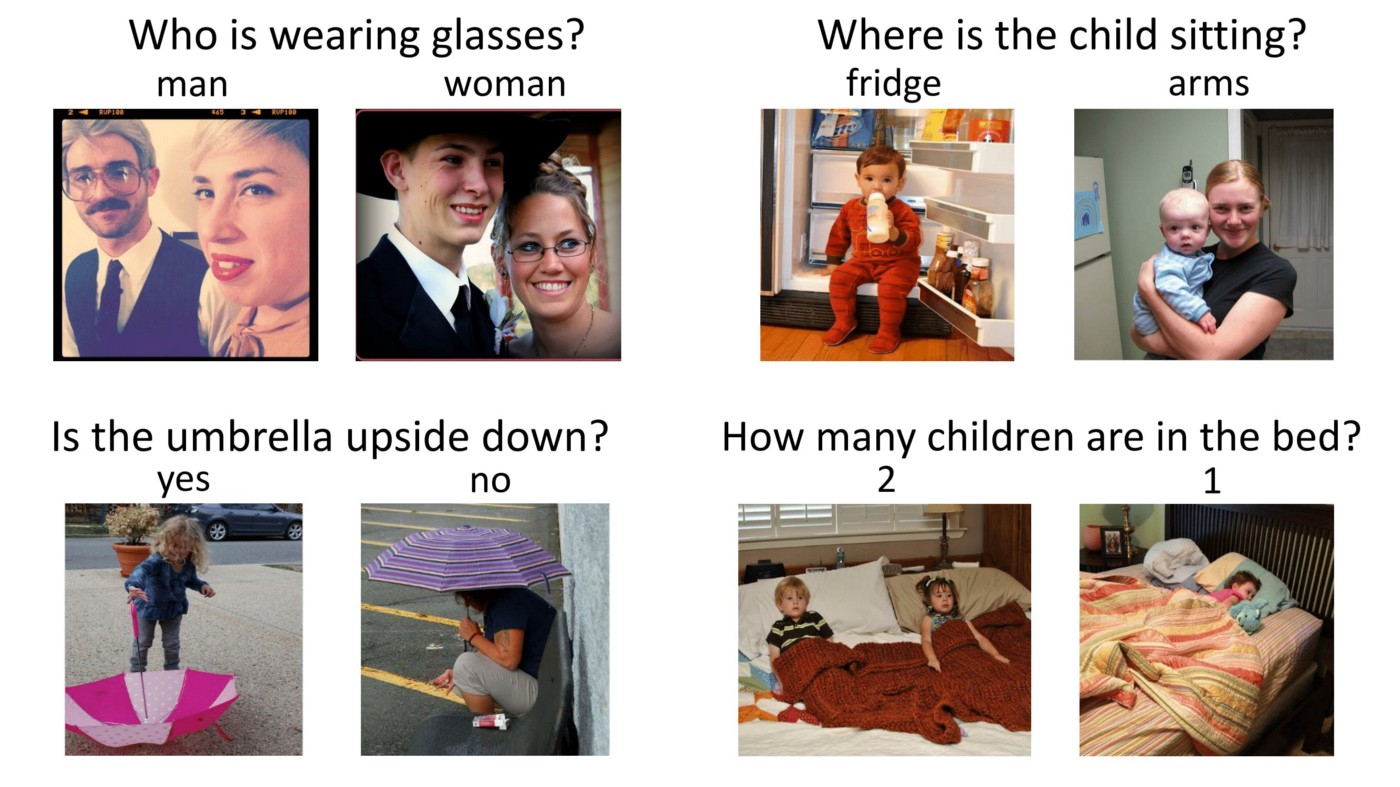
\includegraphics[ scale = 0.2]{images/VQADataset.jpeg}
		\label{figure1}
		\caption{Samples from VQA dataset}
	\end{figure}

\section{Evaluation metric}
The experimental results will be presented in terms of the \textbf{accuracy} of the models over our provided dataset.

\section{Baseline method}
	In this section, we describe the Vanilla VQA model~\cite{Agrawal_2016} which considered as a benchmark for deep learning methods. The Vanilla VQA model uses CNN for feature extraction and LSTM or Recurrent networks for language processing. These features are combined using element-wise operations to a common feature, which is used to classify to one of the answers as shown in figure 2.
	
	\begin{figure}[h!]
		\centering
		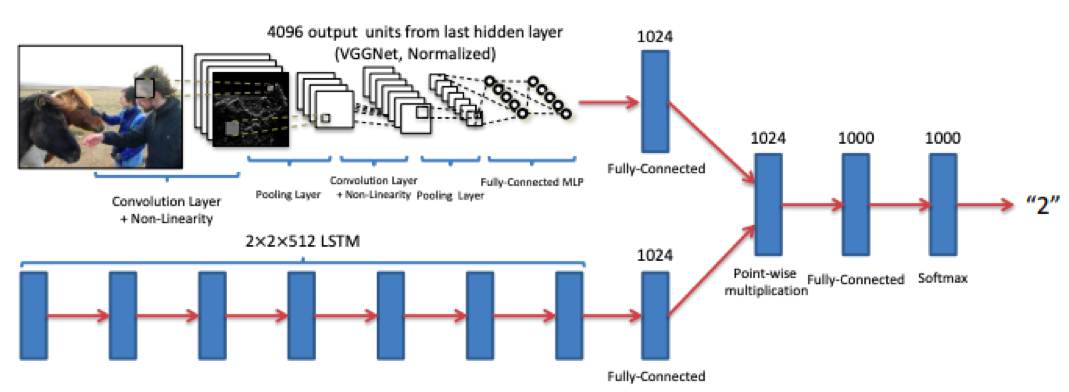
\includegraphics[ scale = 0.8]{images/vanilla.png}
		\label{figure2}
		\caption{Vanilla VQA Network Model~\cite{Agrawal_2016}}
	\end{figure}

	In this project, we try to implement the Vanilla VQA model and report the computation results across our provided dataset. In the following,  According to our time and computational resources, we consider implementing one of the attention-based models such as Stacked Attention Networks~\cite{Yang_2016}, Pythia v1.0~\cite{jiang2018pythia} and the Differential Network~\cite{wu2019differential}(recent method proposed for VQA task that shows very promising performance over different datasets.)
	
\bibliographystyle{abbrv}
\bibliography{bibliography}

\end{document}
